\documentclass[norsk,12pt]{article}
\usepackage[utf8]{inputenc}
\usepackage[T1]{fontenc}

\usepackage{floatpag}				% Different pagestyles
\usepackage{amsmath}
\usepackage{array}	
\usepackage{booktabs}
\usepackage{amssymb}
\usepackage{graphicx}
\usepackage{epstopdf}
\usepackage{tabularx}
\usepackage{float}
\usepackage{caption}
\usepackage{subcaption}
\usepackage{parskip}
\usepackage{multirow}
\usepackage{listings}


\begin{document}
\title{Oblig2}
\author{Magnus Isaksen}
\maketitle

\section*{a)}

For et N-spinn system er totalt antall mikrotilstander gitt ved

$\Omega = \frac{N!}{S!(N-S)!}$

Hvor N er antall mulige spinn tilstander og S er spinn partikler vi er interesserte i. 

\section*{b)}

Med et gjennomsnitts spinn $2s =S_+ - S_-$ vil vi kunne sette dette inn og får den totale energien: 

$E_{tot} = \mu B (S_+ - S_-) = \mu B (S-2s) $

Hvor $S = S_+ + S_-$ er det totale antall spinntilstandene. 

\section*{c)}

Genererer 10000 mikrotilstander for N= 50 som sett i Figur \ref{mikro}

\begin{lstlisting}
from pylab import *

N = 50  
S = 10000
m = randint(-1,2,(N,S))
print(m[0:5,:])
n = sum(m, axis=1)
hist(n)

hold('on')
sn = linspace(-300,300,10000)
plot(sn,exp(-2*sn**2/N), 'r-')
show()
\end{lstlisting}

\begin{figure}[hb!]
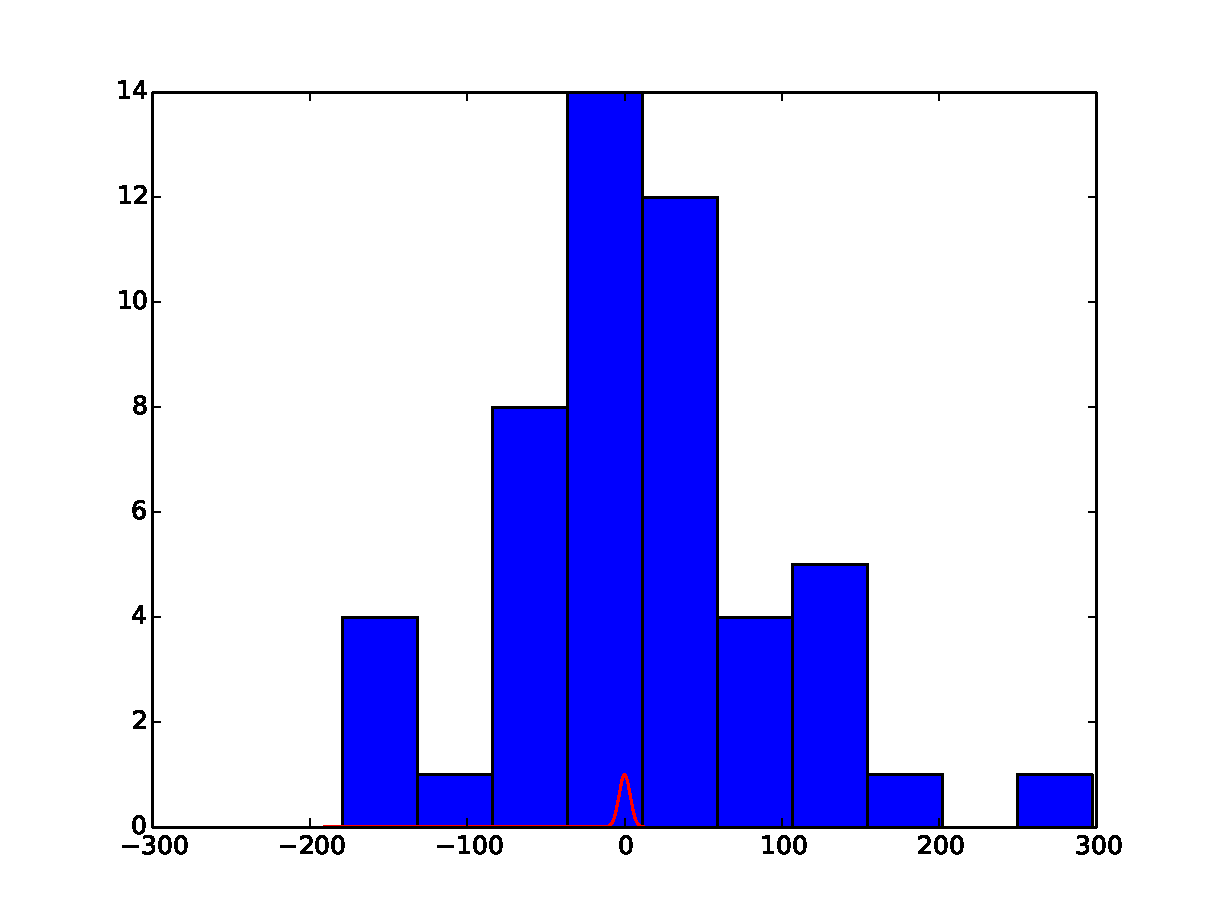
\includegraphics[width = \textwidth]{figure_1.pdf}
\caption{10000 mikrotilstander for N = 50}
\label{mikro}
\end{figure}

\section*{d)}

Setter vi inn med ønske om å finne $S_+$ i formelen for å finne spinntilstander

$\Omega (N,S_+) = \frac{N!}{S_+!(N-S_+)!}$

Vi vet at $N = S_+ + S_-$, noe som gir oss $ N-S_+ = S_-$ 

Og vi får da: 

$\Omega (N,S_+) = \frac{N!}{S_+!S_-!}$

\section*{e)}

Siden jeg vet at 

$ N = S_+ + S_-$ 

og vet at 

$ 2s = S_+-S_-$

kan jeg skrive disse om og sette inn i lignigen i d.

Først for $S_-$

$S_+ = 2s +S_-$ 

$N = 2s+S_- +S_- = 2s +2S_-$

$S_- = \frac{1}{2} N -s$

Så for $S_+$

$S_- = S_+ -2s$

$N = 2S_+ -2s$

$S_+ = \frac{1}{2} N +s$

Setter vi dette inn i uttrykket for $S_+ $ og $S_-$ får vi 

$\Omega (N,s) = \frac{N!}{(\frac{1}{2} N +s)! (\frac{1}{2}N - s)!}$


\section*{f)}

\section*{g)}

Den analytiske og den numeriske ser ut til å sentrere seg rundt samme plass, men den numeriske løsningen er ikke like skarpt midtstilt som den analytiske kurven er. Så det ser ut til at det stemmer bra med den numeriske løsningen. Den røde linja i Figur \ref{mikro} er det analytiske resultatet. 


\section*{h)}

Med spinn $2s = N_+ - N_-$ kan vi få spinn $[0, 1, 2]$. Da hvis atomet har spinn adderes spinnene og de gir bidrag til spinnet ut fra formen på 2s. 

$U = NkT$ hvor N er tilstanden til atomet. Så mulige energier er U = 0.0. U= kT og U = 2kT
 
 
\section*{i)}

Microtilstander til to systemer sammen finner vi ved $\Omega_1*\Omega_2$ hvor $\Omega_1 = \Omega_1(N_1,0)*exp(-\frac{2s_1^2}{N_1})$ Og $\Omega_2 = \Omega_2(N_2,0)*exp(-\frac{2s_2^2}{N_2})$. 

Setter vi disse sammen får vi

$\Omega_1(N_1,0)exp(-\frac{2s_1^2}{N_1})\Omega_2(N_2,0)exp(-\frac{2s_2^2}{N_2}) = \Omega_1(N_1,0)\Omega_2(N_2,0)exp(-\frac{2s_1^2}{N_1}-\frac{2s_2^2}{N_2})$

 
\section*{j)}

Den mest sannsynlige tilstanden er når de er i likevekt. 

Dette finner vi med: 

$\frac{d(\ln{\Omega_1(N_1,0)*exp(-\frac{4s_1}{N_1})}}{dq_1} = \frac{d(\ln{\Omega_2(N_2,0)*exp(-\frac{4s_2}{N_2})}}{dq_2}$

Deriverer med hensyn på q og får

$\ln{exp(-\frac{4s_1}{N_1})} = \ln{exp(-\frac{4s_2}{N_2})}$

$\frac{s_1}{N_1} = \frac{s_2}{N_2}$ 


\section*{k)}

Multiplisiteten til spinn $S_+$ er gitt ved $\Omega (N,S_+) = \frac{N!}{S_+!(N-S_+)!}$

Entropien er gitt ved $S = k \ln{\Omega (N,S_+)}$

Så $S(N,S_+) = k \ln{\frac{N!}{S_+!(N-S_+)!}}$

\section*{l)}

Temperatur er gitt ve $\frac{1}{T} = \frac{dS}{dU}$ og for dette systemet kan vi sette $\frac{1}{T} = \frac{dS}{dS_+}\frac{dS_+}{dU}$ Og $\frac{dS}{dU} = -\frac{1}{2\mu B}$

Slik at uttrykket for temperaturen da er $\frac{1}{T} = -\frac{1}{2\mu B}\frac{dS}{dS_+}$


\end{document}